% Plano de Verificação — riscv-dma-matrix-coprocessor
% Compilar: make pdf  (pdflatex, 3 passadas)
\documentclass[10pt,a4paper]{article}
\usepackage[T1]{fontenc}
\usepackage[utf8]{inputenc}
\usepackage{lmodern}
\usepackage[a4paper,margin=2.5cm]{geometry}
\usepackage{microtype}
\usepackage{amsmath}
\usepackage{booktabs,longtable,array}
\usepackage[table]{xcolor}
\usepackage{fancyhdr}
\usepackage{caption}
\usepackage{enumitem}
\usepackage{graphicx}
% ragged2e não está disponível (falta everysel.sty): margem direita irregular com hifenização
\newcommand{\myrag}{\rightskip=0pt plus 2em \spaceskip=.3333em \xspaceskip=.5em\relax}
\usepackage{tikz}
\usetikzlibrary{arrows.meta,positioning,calc,shapes.geometric,fit}
\usepackage[hidelinks]{hyperref}

% Nomes em português (babel-pt não está instalado no servidor)
\renewcommand{\contentsname}{Sumário}
\renewcommand{\refname}{Referências}
\renewcommand{\figurename}{Figura}
\renewcommand{\tablename}{Tabela}
\hyphenation{ve-ri-fi-ca-ção co-pro-ces-sa-dor ace-le-ra-dor re-gis-tra-do-res re-gis-tra-dor
  con-fi-gu-ra-ção trans-fe-rên-cia trans-fe-rên-cias in-ter-rup-ção sub-sis-te-ma
  pa-ra-me-tri-zá-vel pa-ra-me-tri-za-ção me-mó-ria com-par-ti-lha-da de-co-di-fi-ca-dor
  en-de-re-ça-men-to au-to-no-mia bar-ra-men-to re-gres-são co-ber-tu-ra score-board}

\newcolumntype{L}[1]{>{\myrag\arraybackslash}p{#1}}
\setlength{\emergencystretch}{2em}
\captionsetup{labelfont=bf,font=small,skip=4pt}
\setlist[itemize]{leftmargin=1.6em,itemsep=2pt,topsep=3pt}
\setlist[enumerate]{itemsep=2pt,topsep=3pt}
\definecolor{grp}{gray}{0.90}
\definecolor{tlm}{RGB}{0,140,160}
\definecolor{bar}{RGB}{90,150,210}
\definecolor{ms}{RGB}{170,100,20}
\newcommand{\DW}{\mathit{DW}}
\newcommand{\code}[1]{\texttt{#1}}

\pagestyle{fancy}
\fancyhf{}
\fancyhead[L]{\small Plano de Verificação --- riscv-dma-matrix-coprocessor}
\fancyhead[R]{\small CEPEDI --- CI Digital}
\fancyfoot[C]{\thepage}
\renewcommand{\headrulewidth}{0.4pt}

\hypersetup{pdftitle={Plano de Verificação — riscv-dma-matrix-coprocessor},
  pdfauthor={Gustavo Santiago, Leandro Gama, Valerio Gabriel, Carolina Correia}}

\begin{document}

% ------------------------------------------------------------------ capa
\begin{titlepage}
\centering
\vspace*{4.2cm}
{\LARGE\bfseries Plano de Verificação\par}
\vspace{1.1cm}
{\Large Sistema \code{riscv-dma-matrix-coprocessor}\par}
\vspace{0.5cm}
{CPU RV32I, controlador de DMA, acelerador sistólico \emph{weight-stationary}\\
parametrizável ($N = 2, 4, 8$) e memória compartilhada\par}
\vspace{0.6cm}
{DUTs: \code{accel\_systolic} $\cdot$ \code{accel\_top} $\cdot$ CSR $\cdot$ DMA $\cdot$
memória compartilhada $\cdot$ barramento AXI4-Lite $\cdot$ \code{soc\_top}\par}
\vspace{2.0cm}
{Gustavo Santiago, Leandro Gama, Valerio Gabriel, Carolina Correia\par}
\vspace{0.25cm}
{Equipe do projeto \code{riscv-dma-matrix-coprocessor}\par}
\vspace{1.0cm}
{CEPEDI --- CI Digital\par}
\vspace{0.2cm}
{Programa de Desenvolvimento de Competências em Sistemas Digitais\par}
\vfill
\begin{tabular}{@{}p{2.3cm}L{12.6cm}@{}}
\toprule
Documento & Plano de Verificação (versão inicial)\\
Versão & 0.1\\
Data & 14/11/2026\\
Base & READMEs de \code{02.Architecture}, \code{03.Reference}, \code{04.RTL} e \code{05.Verification};
RTL do acelerador (\code{accel\_top.sv}, \code{accel\_systolic.sv}) e \code{axil\_if.sv};
enunciado do projeto e enunciado do trabalho final de verificação; commit \code{f8fc43c} de 14/11/2026\\
\bottomrule
\end{tabular}
\end{titlepage}

% ------------------------------------------------------------------ sumário
\tableofcontents
\vspace{1.5em}
\section*{Histórico de revisões}
\begin{tabular}{@{}llL{11.4cm}@{}}
\toprule
Versão & Data & Descrição\\
\midrule
0.1 & 14/11/2026 & Versão inicial: introdução, DUTs, metas, plano de teste, cobertura e cronograma
preliminar. Base: RTL do acelerador (E2), golden model e ICD parcial.\\
\bottomrule
\end{tabular}
\clearpage

% ------------------------------------------------------------------ figura 1
\begin{figure}[t]
\centering
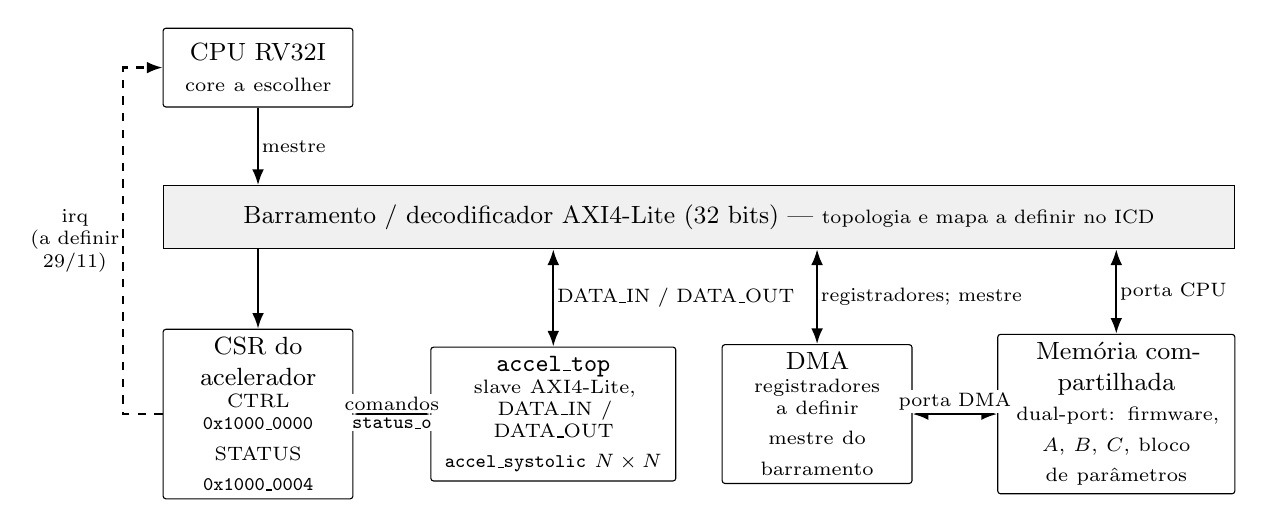
\begin{tikzpicture}[x=1cm,y=1cm,font=\small,
  blk/.style={draw,rounded corners=1pt,align=center,fill=white,inner sep=3pt,minimum height=1.7cm},
  bus/.style={draw,align=center,fill=gray!12,inner sep=3pt},
  arr/.style={-{Latex[length=2mm]},thick},
  darr/.style={{Latex[length=2mm]}-{Latex[length=2mm]},thick},
  lbl/.style={font=\scriptsize,fill=white,inner sep=1pt,align=center}]
\node[blk,text width=2.2cm] (csr) at (1.2,0)
  {CSR do acelerador\\ \scriptsize CTRL \code{0x1000\_0000}\\ \scriptsize STATUS \code{0x1000\_0004}};
\node[blk,text width=2.9cm] (acc) at (4.95,0)
  {\code{accel\_top}\\ \scriptsize slave AXI4-Lite,\\ \scriptsize DATA\_IN / DATA\_OUT\\
   \scriptsize \code{accel\_systolic} $N\times N$};
\node[blk,text width=2.2cm] (dma) at (8.3,0)
  {DMA\\ \scriptsize registradores a definir\\ \scriptsize mestre do barramento};
\node[blk,text width=2.8cm] (mem) at (12.1,0)
  {Memória compartilhada\\ \scriptsize dual-port: firmware, $A$, $B$, $C$, bloco de parâmetros};
\node[bus,minimum width=13.6cm,minimum height=0.8cm] (bus) at (6.8,2.5)
  {Barramento / decodificador AXI4-Lite (32 bits) --- \scriptsize topologia e mapa a definir no ICD};
\node[blk,text width=2.2cm,minimum height=1.0cm] (cpu) at (1.2,4.4)
  {CPU RV32I\\ \scriptsize core a escolher};
\draw[arr] (cpu.south) -- node[lbl,right]{mestre} (cpu.south |- bus.north);
\draw[arr] (csr.north |- bus.south) -- (csr.north);
\draw[darr] (acc.north |- bus.south) -- node[lbl,right]{DATA\_IN / DATA\_OUT} (acc.north);
\draw[darr] (dma.north |- bus.south) -- node[lbl,right]{registradores; mestre} (dma.north);
\draw[darr] (mem.north |- bus.south) -- node[lbl,right]{porta CPU} (mem.north);
\draw[darr] (csr.east) -- node[lbl,above]{comandos} node[lbl,below]{\code{status\_o}} (acc.west);
\draw[darr] (dma.east) -- node[lbl,above]{porta DMA} (mem.west);
\draw[dashed,arr] (csr.west) -- ++(-0.5,0) |- node[lbl,pos=0.25,left]{irq\\(a definir\\29/11)} (cpu.west);
\end{tikzpicture}
\caption{Sistema a verificar. Os comandos do CSR para o acelerador são \code{mode\_i}, \code{load\_i},
\code{start\_i} e \code{clr\_error\_i}; o acelerador devolve \code{status\_o}. Só o acelerador, o CSR
(como contrato) e a interface \code{axil\_if} existem em 14/11/2026; os demais blocos seguem o enunciado
e o roadmap.}
\label{fig:sistema}
\end{figure}

% ------------------------------------------------------------------ 1
\section{Introdução}

\subsection{Visão geral do projeto}

O projeto é um sistema digital que calcula $C = A \times B$. Uma CPU RISC-V RV32I apenas configura
endereços e dimensões e dispara a operação; um controlador de DMA move, de forma autônoma, os blocos de
$A$ e $B$ da memória compartilhada para o buffer de entrada do acelerador, emite os comandos de carga e
de execução e grava os blocos de $C$ de volta na memória; o acelerador é um \emph{systolic array
weight-stationary} $N \times N$ ($N \in \{2, 4, 8\}$) com elementos de \code{DATA\_WIDTH} $\in \{8, 16,
32\}$ bits, acumulador interno de $2\cdot\DW + \lceil \log_2 N \rceil$ bits e saída de $\DW$ bits com
\emph{wrap} (sem saturação). Matrizes maiores que a malha são particionadas em blocos (\emph{tiling})
fora do acelerador. O tráfego de controle usa AXI4-Lite de 32 bits. O término é sinalizado por
registrador de status; a adoção de interrupção será decidida em 29/11/2026. O enunciado exige a síntese
de pelo menos três configurações da malha e um ambiente UVM integrado que compare automaticamente a
matriz $C$ produzida pelo hardware com um modelo de referência.

A verificação se apoia em três fontes de referência:
\begin{enumerate}
  \item o \textbf{golden model em Python} (\code{03.Reference/golden/systolic\_array.py}), modelo
  funcional da multiplicação por blocos, com a mesma máscara de acumulador e o mesmo \emph{wrap} do RTL;
  \item os \textbf{vetores gerados} por \code{generate\_rtl\_vectors.py}: 81 casos (9 configurações
  $N \times \DW$ vezes 9 casos), com seed 2026, em arquivos texto que o testbench lê;
  \item \textbf{modelos de transação em SystemVerilog} para o barramento AXI4-Lite, os registradores
  (CSR e DMA) e a sequência de comandos do acelerador.
\end{enumerate}
Não há co-simulação instrução a instrução do core: ele é verificado pelo seu dono com programas
autoverificáveis e, neste plano, é tratado como o executor do firmware.

\subsection{Descrição dos DUTs}

A Figura~\ref{fig:sistema} mostra o sistema e a Tabela~\ref{tab:niveis} os três níveis em que ele é
verificado. Cada bloco entra no subsistema e no sistema só depois de passar no seu próprio ambiente.

\begin{table}[htbp]
\centering\small
\caption{Níveis de verificação, DUTs e ambientes.}
\label{tab:niveis}
\begin{tabular}{@{}L{1.6cm}L{5.9cm}L{7.4cm}@{}}
\toprule
Nível & DUTs & Ambiente\\
\midrule
N1 Unidade & Acelerador: \code{accel\_systolic} e \code{accel\_top} (slave AXI4-Lite, buffers e
array); golden model; memória compartilhada; CSR do acelerador; DMA isolado (com memória e acelerador
comportamentais); core RV32I isolado. &
Testbenches SystemVerilog dirigidos com tasks e linha \code{RESUMO: n OK, m ERRO}
(\code{05.Verification/unit/}); o do acelerador já existe (\code{accel\_top\_tb.sv}: 9 instâncias
$N \times \DW$, 81 vetores do golden); \code{unittest} Python (\code{make test}); programas
autoverificáveis do core contra memória-modelo.\\
N2 Bloco e subsistema & Acelerador com agente AXI4-Lite UVM (o ambiente faz o papel do DMA, três
valores de $N$); \textbf{subsistema E3}: DMA + memória + CSR + acelerador, sem CPU (o testbench faz o
papel da CPU). &
UVM em \code{05.Verification/subsys/}: agente \code{op} (sequencer, driver A = BFM AXI4-Lite que
programa DMA e CSR, monitor), agente AXI4-Lite passivo, modelo de referência, scoreboard e cobertura;
SVA em arquivos de \code{bind}.\\
N3 Sistema & \code{soc\_top}: CPU + barramento/decodificador + CSR + DMA + memória compartilhada +
acelerador, executando o firmware. &
UVM integrado em \code{05.Verification/soc/}, reaproveitando o ambiente N2: driver B (carga das
memórias por \emph{backdoor} e firmware genérico) por \emph{factory override}; monitor lê $C$ na
memória; agentes de barramento passivos; vetores do golden em arquivo e modelo de referência por TLM.\\
\bottomrule
\end{tabular}
\end{table}

\begin{table}[htbp]
\centering\footnotesize
\setlength{\tabcolsep}{4pt}
\caption{Mapa de endereços: o que está definido e o que falta.}
\label{tab:mapa}
\begin{tabular}{@{}L{2.0cm}L{1.7cm}L{4.3cm}L{1.2cm}L{1.8cm}L{3.4cm}@{}}
\toprule
Base & Tamanho & Região & CPU & DMA & Fonte / situação\\
\midrule
a definir & a definir & Memória de instruções (firmware \code{.hex}) e vetor de reset & busca & --- &
ICD (a definir)\\
a definir & a definir & Memória de dados compartilhada: $A$, $B$, $C$ e bloco de parâmetros &
\code{lw}/\code{sw} & lê $A$ e $B$, escreve $C$ & ICD (a definir); dual-port (\code{04.RTL/soc})\\
\code{0x0000\_0000} & até \code{0x4000\_0000} & ``Faixa de CSR'' declarada em \code{csr\_readme.md} &
--- & --- & \textbf{inconsistente}: sobrepõe as memórias e deixa os buffers de fora (P10)\\
\code{0x1000\_0000} & 4 B & Acelerador CTRL: MODE (bit 0, RW); LOAD, START, CLR\_ERROR (bits 1--3,
W1P) & \code{sw}/\code{lw} & a definir (P9) & \code{csr\_readme.md}; RTL não existe\\
\code{0x1000\_0004} & 4 B & Acelerador STATUS (RO) = \code{status\_o}: STATE[1:0], DONE[2], ERROR[3]
& \code{lw} & a definir & idem\\
\code{0x1000\_0008} a \code{0x2000\_0000} & --- & Reservado ao acelerador & --- & --- &
\code{csr\_readme.md}\\
a definir & a definir & Registradores do DMA: bases de $A$, $B$, $C$; dimensões; CTRL; STATUS &
\code{sw}/\code{lw} & --- & \code{csr\_readme.md}: ``to be defined''\\
\code{0x4000\_1000} & $N^2\cdot\DW/8$ B (4 a 256) & \code{accel\_top} DATA\_IN (só escrita; OKAY só
em IDLE) & --- & escrita & parâmetro \code{DATA\_IN\_BASE}\\
\code{0x4000\_2000} & $N^2\cdot\DW/8$ B & \code{accel\_top} DATA\_OUT (só leitura; aceita em qualquer
estado) & --- & leitura & parâmetro \code{DATA\_OUT\_BASE}\\
qualquer outro & --- & Resposta a definir (proposta: SLVERR/DECERR no decodificador) & & & ICD (a
definir)\\
\bottomrule
\end{tabular}
\end{table}

\paragraph{Acelerador.}
A casca \code{accel\_top} tem um slave AXI4-Lite de 32 bits (\code{axil\_if.target}), um buffer de
entrada \code{input\_q} de \code{BUFFER\_WORDS} $= N^2\cdot\DW/32$ palavras e um buffer de saída
\code{output\_words}, que é um apelido dos registradores \code{result\_q} do array. Admite uma escrita
e uma leitura pendentes; \code{bvalid} sobe um ciclo após o último handshake de AW/W e \code{rvalid}
um ciclo após o de AR; \code{wstrb} habilita bytes; respondem SLVERR o endereço desalinhado, o
endereço fora da faixa, a escrita fora de IDLE, a escrita em DATA\_OUT e a leitura de DATA\_IN;
\code{awprot}/\code{arprot} são ignorados e os erros AXI não alteram o bit ERROR. O núcleo
\code{accel\_systolic} tem a FSM IDLE (\code{00}) / LOADING (\code{01}) / PROCESSING (\code{10}):
LOAD só é aceito em IDLE com \code{mode\_i}=0 e START só em IDLE com \code{mode\_i}=1, nunca os dois
juntos; qualquer outro LOAD/START liga ERROR (\code{status\_o[3]}), pegajoso até \code{clr\_error\_i};
DONE (\code{status\_o[2]}) é limpo na aceitação e ligado ao fim. LOADING dura $N$ ciclos (a linha $r$
de $B$ entra no ciclo $r$); PROCESSING dura $3N-2$ ciclos e $C[i][j]$ é capturado no ciclo
$i+N-1+j$; o acumulador tem $2\cdot\DW+\lceil\log_2 N\rceil$ bits e a saída guarda os $\DW$ bits
baixos. Os pesos persistem entre STARTs. Não há interrupção.

\paragraph{CSR do acelerador.}
Contrato em \code{02.Architecture/icd/csr\_readme.md}: CTRL e STATUS de 32 bits; MODE retido;
LOAD, START e CLR\_ERROR geram um pulso de um ciclo por transação (W1P). O RTL não existe e o dono do
bloco não está definido.

\paragraph{DMA.}
Requisitos da seção 5 do enunciado: registradores de endereço-base, dimensões, controle e status;
FSM de leitura de $A$ e $B$, escrita de $C$ e contadores de endereço; operação independente da CPU
após a configuração; coordenação com o acelerador por sinais de requisição, pronto/ocupado e
conclusão. O RTL está previsto para 17--18/11 e os registradores estão ``a definir''.

\paragraph{Memória compartilhada e barramento.}
Memória dual-port (porta da CPU e porta do DMA) e decodificador/interconexão AXI4-Lite. Só existe a
interface genérica \code{axil\_if.sv} (sinais AW, W, B, AR, R e modports \code{initiator}/\code{target}).

\paragraph{CPU e firmware.}
Core RV32I (escolha pendente, por ADR: próprio ou de terceiros) e firmware \emph{freestanding} que lê
um bloco de parâmetros, programa DMA e CSR por ponteiros \code{volatile} de um header gerado do ICD,
dispara a operação e espera o término. O \code{.hex} é versionado em \code{06.Firmware/}.

\paragraph{Golden model.}
A função \code{systolic\_array} recebe \code{a}, \code{b}, \code{array\_size}, \code{data\_width} e
\code{signed}; multiplica por blocos em $M$, $P$ e $K$, mascara o acumulador a $2\cdot\DW + \lceil\log_2 K\rceil$ bits (igual ao RTL quando $K = N$) e
aplica \emph{wrap} em $\DW$ bits na saída; aceita operandos com e sem sinal; 11 testes
\code{unittest}. \code{generate\_rtl\_vectors.py} gera os 81 casos \code{known}, \code{identity},
\code{zero\_weights}, \code{numeric\_limits}, \code{output\_wrap}, \code{random\_load},
\code{random\_reuse}, \code{zero\_input\_reuse} e \code{random\_reuse\_again} (seed
$2026 + 100\cdot N + \DW$), só $N \times N$ e com sinal.

\begin{table}[htbp]
\centering\small
\caption{Estado de cada bloco na data deste plano.}
\label{tab:estado}
\begin{tabular}{@{}L{3.0cm}L{5.2cm}L{6.8cm}@{}}
\toprule
Bloco & RTL & Verificação existente\\
\midrule
Acelerador (\code{accel\_systolic}, \code{accel\_top}) & completo para $N \in \{2,4,8\}$ e $\DW \in
\{8,16,32\}$; sem IRQ; porta de interface e FSM + datapath no mesmo módulo (P13) &
\code{accel\_top\_tb.sv}: SV dirigido, 9 instâncias paralelas, BFM AXI4-Lite com ordem AW/W e
backpressure fixa, casos SLVERR/ERROR, 81 vetores (seed 2026), reset no meio de transação; roda em
Vivado xsim (\code{run\_accel.sh}), não em \code{xrun}; sem SVA, cobertura ou UVM\\
CSR do acelerador & não iniciado (contrato em \code{csr\_readme.md}) & ---\\
DMA & não iniciado (RTL em 17--18/11); registradores a definir & ---\\
Memória compartilhada & não iniciada & ---\\
Barramento / decodificador & não iniciado; só \code{axil\_if.sv} & ---\\
CPU RV32I & core não escolhido; entrega em 24/11 & --- (programas autoverificáveis planejados)\\
Firmware & não iniciado; entrega em 25/11 & ---\\
\code{soc\_top} & não iniciado & ---\\
Golden model (Python) & completo (tiling, wrap, 9 configurações) & 11 testes \code{unittest}
(\code{make test}); gerador de 81 vetores\\
Infraestrutura & --- & \code{env\_smoke} (UVM) prova Xcelium + UVM + licença; \code{uvm\_verdict.sh},
\code{elab\_check.sh}; \code{make check/test/lint/elab-smoke/sim-smoke} com \code{SEED} e
\code{TEST}\\
\bottomrule
\end{tabular}
\end{table}

\subsection{Objetivos e metas da verificação}

\paragraph{Objetivo geral.}
Mostrar, com evidência reproduzível (comando, seed e log), que cada bloco implementa o seu contrato
(READMEs e ICD) e que o sistema integrado, a partir do firmware executado na CPU, calcula
$C = A \times B$ igual ao golden model para várias dimensões e valores, com o DMA operando de forma
autônoma, nas três configurações de malha, por meio de um ambiente UVM 1.2 com checagem automática e
cobertura funcional, conforme o enunciado do trabalho final de verificação.

\paragraph{Objetivos específicos.}
\begin{enumerate}[label=\textbf{O\arabic*.},leftmargin=2.6em]
  \item Verificar cada unidade isoladamente antes da integração: acelerador (testbench existente,
  portado para \code{xrun} e estendido), CSR, memória, DMA e core, com testbenches do dono de cada
  bloco.
  \item Acelerador: equivalência bit a bit de DATA\_OUT com o golden para as 9 configurações
  $N \times \DW$, incluindo limites numéricos, \emph{wrap}, reuso de pesos, backpressure AXI4-Lite
  e todos os casos negativos (SLVERR, ERROR).
  \item CSR e barramento: decodificação do mapa, semântica W1P/RW/RO, respostas de erro e ausência
  de efeitos colaterais.
  \item DMA: FSM completa, endereçamento de $A$, $B$ e $C$, \emph{tiling} (incluindo $K > N$),
  sequência correta de comandos ao acelerador, autonomia e tratamento de erro.
  \item Subsistema E3 (DMA + memória + CSR + acelerador, sem CPU): multiplicação ponta a ponta com
  o testbench no papel da CPU; regressão por seeds $\times$ $N$.
  \item Sistema E4: o firmware configura e dispara; $C$ na memória igual ao golden; término por
  STATUS (e IRQ, se adotada); nenhuma transferência elemento a elemento pela CPU; regressão nas três
  configurações selecionáveis na linha de comando.
  \item Ambiente UVM conforme o enunciado: transação, biblioteca de sequences, agente com objeto de
  configuração, TLM, scoreboard elemento a elemento, cobertura amostrada do monitor com \code{cross},
  testes por \code{+UVM\_TESTNAME}, factory, veredito \code{TEST PASS}/\code{TEST FAIL}; driver A
  (BFM) e driver B (firmware) intercambiáveis por \emph{factory override}; itens opcionais
  (reference model por TLM, monitor de barramento, latência).
  \item Medir e fechar cobertura funcional e de código por bloco, com merge da regressão no IMC e
  exclusões justificadas.
  \item Provar que o ambiente detecta erros (injeção de falhas com \code{TEST FAIL}) e que toda
  espera tem timeout.
  \item Medir ciclos por operação (LOAD, PROCESSING, operação completa) por configuração, para o
  comparativo de desempenho do relatório, sem critério de aprovação.
\end{enumerate}

\begin{table}[htbp]
\centering\small
\caption{Metas quantitativas (critérios de encerramento).}
\label{tab:metas}
\begin{tabular}{@{}L{10.6cm}L{4.8cm}@{}}
\toprule
Métrica & Meta\\
\midrule
Features da Tabela~\ref{tab:features} de prioridade A com teste associado e aprovado & 100\,\%\\
Features de prioridade M com teste aprovado & $\geq$ 90\,\% (restante justificado)\\
\code{accel\_top\_tb}: configurações $N \times \DW$ aprovadas & 9/9 (\code{RESUMO: 9 OK, 0 ERRO})
com seed 2026 e $\geq$ 2 seeds adicionais\\
Divergências acelerador $\times$ golden na regressão aleatória UVM ($\geq$ 300 operações por $N$
com $\DW = 8$; $\geq$ 50 por configuração com $\DW = 16$ e 32) & 0\\
Divergências subsistema (DMA + memória + acelerador) $\times$ golden ($\geq$ 100 operações
aleatórias por $N$, com múltiplos tiles e $K > N$) & 0\\
Divergências sistema (firmware) $\times$ golden ($\geq$ 50 operações aleatórias por $N$ mais todos
os dirigidos) & 0\\
Regressão final: testes $\times$ $\geq$ 10 seeds $\times$ 3 valores de $N$ & 100\,\% \code{TEST
PASS}; \code{UVM\_ERROR : 0}; \code{UVM\_FATAL : 0}\\
Operações pendentes no scoreboard ao fim de cada teste & 0\\
Cobertura funcional (covergroups da Seção~\ref{sec:cobertura}) & 100\,\% (exclusões justificadas)\\
Cobertura de linha/bloco: acelerador, CSR, DMA, memória, decodificador, \code{soc\_top} &
$\geq$ 95\,\%\\
Cobertura de linha do core RV32I & $\geq$ 80\,\% se core próprio; excluída se IP de terceiros\\
Cobertura de FSM (\code{accel\_systolic}, DMA, CSR): estados e transições & 100\,\%\\
Cobertura de toggle nas portas e registradores de controle & $\geq$ 90\,\%\\
Falhas de SVA e de checkers de protocolo na regressão & 0\\
Falhas injetadas ($\geq$ 3 mecanismos) detectadas pelo scoreboard com \code{TEST FAIL} & 100\,\%\\
Simulações travadas (espera sem timeout) na regressão & 0\\
Pontos de atenção P1--P19 com decisão registrada (ADR) & 100\,\% até o fim da S2\\
Bugs abertos de severidade alta & 0\\
Latência medida (ciclos) por configuração e dimensão de teste & registrada (sem critério)\\
\bottomrule
\end{tabular}
\end{table}

\paragraph{Fora do escopo.}
Temporização, área e $f_{\max}$ (cobertas pela síntese no Genus); potência; verificação física;
gate-level e LEC (o Conformal está instalado, mas não é exigido); verificação formal além de lint e
elaboração; conformidade completa do core RV32I (riscv-tests, riscv-arch-test, co-simulação com o
Spike): o core é verificado pelo seu dono e, se for IP de terceiros, tratado como confiável, só a
integração é verificada; $\DW = 16$ e 32 nos níveis N2 e N3 (só no N1); saturação (o projeto define
\emph{wrap}); múltiplos domínios de clock (clock único); desempenho como critério de aprovação.

\subsection{Ambiente e ferramentas}

\begin{itemize}
  \item \textbf{Simulação:} Cadence Xcelium 25.03 (\code{xrun -uvm}, UVM 1.2 da distribuição; o
  README cita 24.09 e será corrigido), SystemVerilog e SVA; formas de onda no SimVision. Flags atuais
  do Makefile: \code{-uvm -access +rwc -timescale 1ns/1ps}, \code{-svseed \$(SEED)},
  \code{+UVM\_TESTNAME=\$(TEST)}.
  \item \textbf{Cobertura:} Cadence IMC (Verisium Manager 25.09): \code{-coverage all}, merge da
  regressão, exclusões versionadas no repositório.
  \item \textbf{Modelo de referência:} golden model Python 3.9 (só biblioteca padrão) e
  \code{generate\_rtl\_vectors.py} (arquivos texto em hexadecimal lidos com \code{\$fscanf}); função
  SystemVerilog de referência (acumulação e \emph{wrap} em $\DW$ bits) para o aleatório restrito,
  validada contra os vetores Python; opcionalmente, porte em C do golden ligado por DPI-C.
  \item \textbf{Software:} GCC RISC-V (\code{-march=rv32i -mabi=ilp32}, \emph{freestanding});
  \textbf{não há toolchain RISC-V no servidor da disciplina}, por isso o \code{.hex} é versionado em
  \code{06.Firmware/}; header do mapa de registradores gerado do ICD.
  \item \textbf{Lint:} Verible (\code{.rules.verible\_lint}: \code{always-ff-non-blocking},
  \code{signal-name-style}, parâmetros em maiúsculas, linhas de 100 colunas) a cada commit;
  elaboração com \code{elab\_check.sh} (falha em \code{*E}, \code{*F} e \code{*W,CUVMPW}).
  \item \textbf{Complementar:} Vivado xsim só como legado do testbench unitário até o porte;
  Genus 25.1 para a síntese (fora do escopo); \code{uvm\_verdict.sh} (\code{SIM PASS} com
  \code{UVM\_ERROR : 0} e \code{UVM\_FATAL : 0}); novos alvos do Makefile \code{sim-accel},
  \code{sim-subsys}, \code{sim-soc}, \code{regress} e \code{cov-merge}.
\end{itemize}

A Figura~\ref{fig:ambientes} mostra os dois ambientes UVM. Os componentes são escritos uma vez e
reaproveitados: a transação, o monitor, o modelo de referência, o scoreboard e a cobertura são os
mesmos no subsistema e no sistema; só o driver muda, por \emph{factory override}. A
Tabela~\ref{tab:uvmreq} relaciona cada requisito do enunciado ao componente que o atende.

\begin{figure}[htbp]
\centering
\begin{minipage}[t]{0.49\textwidth}\centering
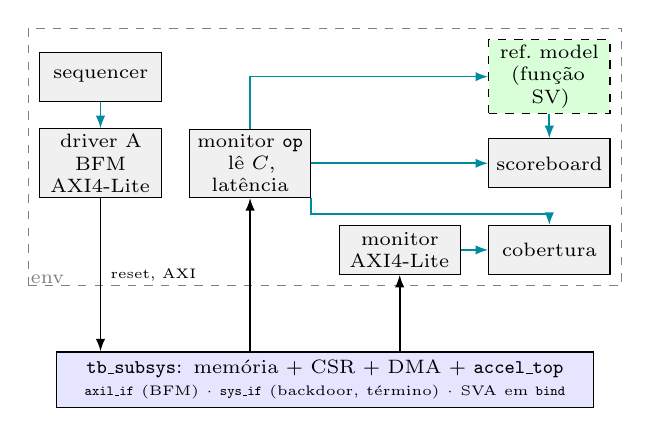
\begin{tikzpicture}[x=1cm,y=1cm,
  every node/.style={font=\scriptsize,align=center},
  agt/.style={draw,fill=gray!12,inner sep=2pt,minimum height=0.62cm,text width=1.4cm},
  ref/.style={draw,dashed,fill=green!15,inner sep=2pt,minimum height=0.62cm,text width=1.4cm},
  dut/.style={draw,fill=blue!10,inner sep=3pt},
  env/.style={draw,dashed,gray,inner sep=4pt},
  a/.style={-{Latex[length=1.6mm]},semithick},
  t/.style={-{Latex[length=1.6mm]},semithick,tlm}]
\node[agt] (seq) at (1.05,4.4) {sequencer};
\node[agt] (drv) at (1.05,3.3) {driver A\\BFM AXI4-Lite};
\node[agt] (mon) at (2.95,3.3) {monitor \code{op}\\lê $C$, latência};
\node[agt] (axm) at (4.85,2.2) {monitor\\AXI4-Lite};
\node[ref] (ref) at (6.75,4.4) {ref.\ model\\(função SV)};
\node[agt] (scb) at (6.75,3.3) {scoreboard};
\node[agt] (cov) at (6.75,2.2) {cobertura};
\node[env,fit=(seq)(drv)(mon)(axm)(ref)(scb)(cov),label={[gray,anchor=south west,inner sep=1pt]south west:env}] {};
\node[dut,text width=6.6cm] (dut) at (3.9,0.55)
  {\code{tb\_subsys}: memória + CSR + DMA + \code{accel\_top}\\
  {\tiny \code{axil\_if} (BFM) $\cdot$ \code{sys\_if} (backdoor, término) $\cdot$ SVA em \code{bind}}};
\draw[t] (seq) -- (drv);
\draw[a] (drv.south) -- node[right]{\tiny reset, AXI} (drv.south |- dut.north);
\draw[a] (mon.south |- dut.north) -- (mon.south);
\draw[a] (axm.south |- dut.north) -- (axm.south);
\draw[t] (mon) -- (scb);
\draw[t] (mon.north) |- (ref.west);
\draw[t] (mon.south east) ++(0,0.0) -- ++(0,-0.2) -| (cov.north);
\draw[t] (axm) -- (cov);
\draw[t] (ref) -- (scb);
\end{tikzpicture}\\[2pt]
{\small \textbf{(a)} Subsistema E3: o testbench faz o papel da CPU.}
\end{minipage}\hfill
\begin{minipage}[t]{0.49\textwidth}\centering
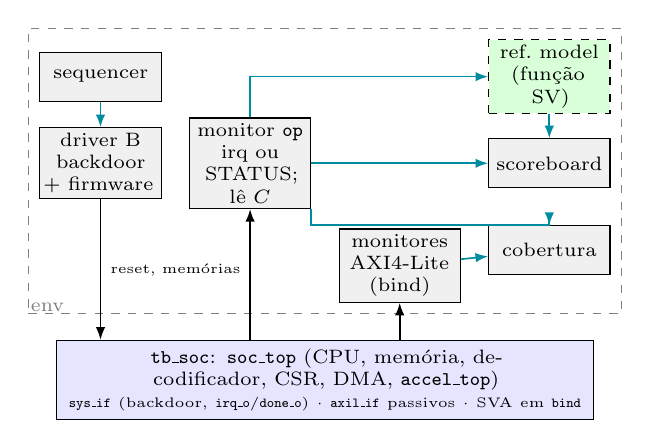
\begin{tikzpicture}[x=1cm,y=1cm,
  every node/.style={font=\scriptsize,align=center},
  agt/.style={draw,fill=gray!12,inner sep=2pt,minimum height=0.62cm,text width=1.4cm},
  ref/.style={draw,dashed,fill=green!15,inner sep=2pt,minimum height=0.62cm,text width=1.4cm},
  dut/.style={draw,fill=blue!10,inner sep=3pt},
  env/.style={draw,dashed,gray,inner sep=4pt},
  a/.style={-{Latex[length=1.6mm]},semithick},
  t/.style={-{Latex[length=1.6mm]},semithick,tlm}]
\node[agt] (seq) at (1.05,4.4) {sequencer};
\node[agt] (drv) at (1.05,3.3) {driver B\\backdoor + firmware};
\node[agt] (mon) at (2.95,3.3) {monitor \code{op}\\irq ou STATUS;\\lê $C$};
\node[agt] (axm) at (4.85,2.0) {monitores\\AXI4-Lite (bind)};
\node[ref] (ref) at (6.75,4.4) {ref.\ model\\(função SV)};
\node[agt] (scb) at (6.75,3.3) {scoreboard};
\node[agt] (cov) at (6.75,2.2) {cobertura};
\node[env,fit=(seq)(drv)(mon)(axm)(ref)(scb)(cov),label={[gray,anchor=south west,inner sep=1pt]south west:env}] {};
\node[dut,text width=6.6cm] (dut) at (3.9,0.55)
  {\code{tb\_soc}: \code{soc\_top} (CPU, memória, decodificador, CSR, DMA, \code{accel\_top})\\
  {\tiny \code{sys\_if} (backdoor, \code{irq\_o}/\code{done\_o}) $\cdot$ \code{axil\_if} passivos $\cdot$ SVA em \code{bind}}};
\draw[t] (seq) -- (drv);
\draw[a] (drv.south) -- node[right]{\tiny reset, memórias} (drv.south |- dut.north);
\draw[a] (mon.south |- dut.north) -- (mon.south);
\draw[a] (axm.south |- dut.north) -- (axm.south);
\draw[t] (mon) -- (scb);
\draw[t] (mon.north) |- (ref.west);
\draw[t] (mon.south east) -- ++(0,-0.2) -| (cov.north);
\draw[t] (axm) -- (cov);
\draw[t] (ref) -- (scb);
\end{tikzpicture}\\[2pt]
{\small \textbf{(b)} Sistema E4: driver B por \emph{factory override}.}
\end{minipage}
\caption{Ambientes UVM. Cinza: componentes UVM; verde tracejado: modelo de referência (opcional como
componente, obrigatório como função do scoreboard); azul: módulos do \code{top\_tb}. Setas em ciano são
conexões TLM. As únicas referências hierárquicas ficam no \code{top\_tb} e nas interfaces; as classes
só enxergam o \emph{virtual interface}.}
\label{fig:ambientes}
\end{figure}

\begin{table}[htbp]
\centering\small
\setlength{\tabcolsep}{4pt}
\caption{Requisitos do enunciado do trabalho final e componentes que os atendem.}
\label{tab:uvmreq}
\begin{tabular}{@{}L{2.6cm}L{11.4cm}L{1.3cm}@{}}
\toprule
Requisito & Componente previsto & Nível\\
\midrule
Transação & \code{op\_item} (\code{uvm\_sequence\_item}): \code{rand} $M$, $K$, $P$, $A$, $B$,
bases e seed, com constraints; \code{convert2string} e \code{do\_compare}; campos de resposta
$C$ observada e \code{latency\_cycles}. & N2, N3\\
Sequences & \code{op\_seq\_lib}: \code{op\_smoke\_seq}, \code{op\_vectors\_seq} (lê os arquivos do
golden), \code{op\_tiling\_seq}, \code{op\_rand\_seq}, \code{op\_errors\_seq}, com
\code{start\_item}/\code{randomize}/\code{finish\_item}. & N2, N3\\
Sequencer & \code{op\_sequencer} (\code{uvm\_sequencer\#(op\_item)}), criado pelo agente e
conectado ao driver no \code{connect\_phase}. & N2, N3\\
Driver & \code{op\_driver\_bfm} (A: programa DMA e CSR por AXI4-Lite) e \code{op\_driver\_fw} (B:
carrega memórias por backdoor com o sistema em reset, libera o reset, espera o término); vif obtido
no \code{uvm\_config\_db}. & N2 / N3\\
Monitor & \code{op\_monitor}: detecta início e fim (START no barramento ou marcador; \code{irq} ou
STATUS.DONE), lê $C$ da memória por backdoor, mede a latência e publica no \code{analysis\_port};
não consulta driver nem sequence. & N2, N3\\
Agente & \code{op\_agent} com \code{op\_cfg} (vif, \code{is\_active}, \code{ARRAY\_SIZE},
\code{DATA\_WIDTH}, timeout). & N2, N3\\
TLM & \code{seq\_item\_port}; \code{analysis\_port} do monitor para \code{op\_ref\_model},
\code{op\_scoreboard} (\code{uvm\_tlm\_analysis\_fifo}) e \code{op\_coverage}; nenhum acesso por
handle direto. & N2, N3\\
Scoreboard & \code{op\_scoreboard}: compara $C$ elemento a elemento, \code{uvm\_error} com linha,
coluna, esperado e obtido; \code{check\_phase} acusa pendências; resumo final. & N2, N3\\
Cobertura funcional & \code{op\_coverage} e \code{axil\_coverage} (\code{uvm\_subscriber}),
amostradas das transações do monitor; Tabela~\ref{tab:covergroups}. & N2, N3\\
Env e testes & \code{subsys\_env}/\code{soc\_env}; \code{op\_base\_test} (\code{+UVM\_TESTNAME},
\code{+ARRAY\_SIZE}, \code{+ERR\_INJECT}, timeout) e testes T09--T24; criação pela factory. &
N2, N3\\
Execução & Makefile: \code{sim-subsys}, \code{sim-soc}, \code{regress} com \code{SEED}, \code{TEST},
\code{N} e \code{COV=1}; veredito \code{TEST PASS}/\code{TEST FAIL} no \code{report\_phase},
validado por \code{uvm\_verdict.sh}. & todos\\
Opcionais & \code{op\_ref\_model} por TLM; \code{axil\_agent} passivo (monitor de barramento e
autonomia); \code{+ARRAY\_SIZE} com três valores na regressão; \code{latency\_cycles} na transação. &
N2, N3\\
\bottomrule
\end{tabular}
\end{table}

\paragraph{Infraestrutura que ainda não existe e é pré-requisito.}
(i) Alvo \code{make sim-accel} com o testbench do acelerador em \code{xrun} e cobertura (hoje só
Vivado). (ii) Agente AXI4-Lite UVM reaproveitável (driver, monitor, config e SVA em \code{bind}) em
\code{05.Verification/common/vip/}. (iii) Gerador de casos $(M, K, P)$ com imagem de memória e bloco
de parâmetros, além dos 81 vetores $N \times N$. (iv) Função SystemVerilog de referência e,
opcionalmente, porte em C do golden para DPI-C. (v) RTL do CSR e modelos comportamentais de DMA e CPU
(sprint 2.3 do roadmap), para começar antes do RTL real. (vi) \code{top\_tb} com interface de
\emph{backdoor} para as memórias e sinal observável de término (P8). (vii) Script de regressão
(testes $\times$ seeds $\times$ $N$) com merge no IMC e tabela de vereditos. (viii) Firmware genérico,
header gerado do ICD e \code{.hex} versionado.

% ------------------------------------------------------------------ 2
\section{Plano de teste}

\subsection{Features a serem verificadas}

A Tabela~\ref{tab:features} lista as features extraídas do RTL, dos READMEs e do enunciado.
Métodos: \textbf{D} = teste dirigido, \textbf{R} = aleatório restrito, \textbf{A} = asserção,
\textbf{M} = comparação com modelo de referência, \textbf{C} = cobertura funcional, \textbf{G} =
netlist (LEC ou gate-level), \textbf{F} = checagem estrutural (lint, elaboração, revisão).
Prioridade: \textbf{A}lta, \textbf{M}édia, \textbf{B}aixa. Os identificadores P$n$ remetem aos
pontos de atenção da Seção~\ref{sec:pontos}.

{\small\setlength{\tabcolsep}{4pt}
\begin{longtable}{@{}L{1.35cm}L{2.45cm}L{8.3cm}L{1.25cm}L{0.55cm}@{}}
\caption{Features a serem verificadas.}\label{tab:features}\\
\toprule
ID & Feature & Comportamento esperado / critério & Método & Pri.\\
\midrule
\endfirsthead
\caption[]{Features a serem verificadas (continuação).}\\
\toprule
ID & Feature & Comportamento esperado / critério & Método & Pri.\\
\midrule
\endhead
\midrule
\multicolumn{5}{r}{\footnotesize continua na próxima página}\\
\endfoot
\bottomrule
\endlastfoot
\rowcolor{grp}\multicolumn{5}{@{}l}{\textbf{Acelerador (\code{accel\_top} / \code{accel\_systolic})}}\\
ACC-01 & Reset & Com \code{rst\_ni}=0: \code{status\_o}=0 (IDLE, DONE=0, ERROR=0),
\code{awready}=\code{wready}=\code{arready}=0, \code{bvalid}=\code{rvalid}=0, \code{input\_q},
\code{weight\_q} e \code{result\_q} zerados. Reset assíncrono com AW aceito sem W, ou com
\code{rvalid} pendente, descarta a transação; depois escrita e leitura funcionam; sem X nas saídas
após o reset. & D, A & A\\
ACC-02 & Handshake AXI4-Lite & Transferência quando VALID e READY estão em 1 na borda; AW e W
aceitos em qualquer ordem (W antes de AW, AW antes de W, juntos) e de forma independente; a escrita
efetiva uma única vez (\code{write\_commit}) após ambos; \code{bvalid} sobe exatamente 1 ciclo após
o último handshake; \code{rvalid} sobe 1 ciclo após o handshake de AR. & D, R, A & A\\
ACC-03 & Uma pendente por canal; backpressure & \code{awready}/\code{wready}=0 enquanto houver AW/W
pendente ou \code{bvalid}=1; \code{arready}=0 enquanto \code{rvalid}=1; \code{bresp}/\code{bvalid}
e \code{rdata}/\code{rresp}/\code{rvalid} estáveis até \code{bready}/\code{rready} (atraso de 0 a
$n$ ciclos). & D, R, A & A\\
ACC-04 & Decodificação de DATA\_IN & Escrita alinhada em [\code{DATA\_IN\_BASE}, $+N^2\cdot\DW/8$)
com STATE=IDLE: OKAY e \code{input\_q[(awaddr-base)>>2]} atualizado; elementos em little-endian
($32/\DW$ por palavra), posição $(\text{endereço}-\text{base})/(\DW/8)$. & D, R, M & A\\
ACC-05 & Byte strobes & Só os bytes com \code{wstrb[lane]}=1 são escritos; \code{wstrb}=0 responde
OKAY sem efeito; reconstrução byte a byte de uma palavra; strobes parciais em palavras diferentes de
0. & D, R & A\\
ACC-06 & Erros de escrita & SLVERR (\code{2'b10}) para \code{awaddr[1:0]}$\neq$0, offset $\geq$
\code{BUFFER\_BYTES}, endereço abaixo da base, escrita em DATA\_OUT ou STATE$\neq$IDLE
(LOADING/PROCESSING); buffer preservado; \code{status\_o[3]} (ERROR) não é afetado. & D, R & A\\
ACC-07 & Leitura de DATA\_OUT & Leitura alinhada em [\code{DATA\_OUT\_BASE}, $+$\code{BUFFER\_BYTES}):
OKAY com \code{rdata}=\code{output\_words[idx]}, capturado no handshake de AR; empacotamento igual
ao de DATA\_IN. & D, M & A\\
ACC-08 & Erros de leitura; \code{awprot}/\code{arprot} & SLVERR com \code{rdata}=0 para
desalinhado, fora da faixa ou em DATA\_IN; leituras aceitas em qualquer estado;
\code{awprot}/\code{arprot} sem efeito na resposta (P7). & D, R & A\\
ACC-09 & Comando LOAD & Aceito só com IDLE, \code{mode\_i}=0, \code{load\_i}=1, \code{start\_i}=0;
vai a LOADING e limpa DONE no ciclo da aceitação; \code{weight\_q[r][*]} $\leftarrow$
\code{data\_i[r*N+*]} no ciclo $r$; LOADING dura $N$ ciclos; volta a IDLE com DONE=1. &
D, M, A, C & A\\
ACC-10 & Comando START & Aceito só com IDLE, \code{mode\_i}=1, \code{start\_i}=1, \code{load\_i}=0;
PROCESSING dura $3N-2$ ciclos (\code{LAST\_CYCLE}=$3N-3$); DONE=1 e IDLE ao final; DONE=1 não
bloqueia novo comando. & D, A, C & A\\
ACC-11 & Comando inválido & \code{load\_i}/\code{start\_i} com \code{mode\_i} errado, ambos em 1,
ou fora de IDLE (LOAD ou START durante LOADING e durante PROCESSING): ERROR=1 pegajoso, sem mudança
de estado, de DONE nem do resultado em curso. & D, R, A & A\\
ACC-12 & CLR\_ERROR & \code{clr\_error\_i}=1 limpa ERROR; se coincidir com comando inválido no
mesmo ciclo, o \emph{set} prevalece (ERROR permanece 1), a confirmar no ICD (P5). & D, A & M\\
ACC-13 & Produto de um tile & DATA\_OUT igual ao golden para os casos \code{known},
\code{identity}, \code{zero\_weights} e \code{random\_load} nas 9 configurações
$N \in \{2,4,8\} \times \DW \in \{8,16,32\}$. & D, R, M & A\\
ACC-14 & Sinal, limites e wrap & Complemento de dois; $(-2^{\DW-1}) \times (-2^{\DW-1})$,
máx$\,\times\,$máx, máx$\,\times\,$mín; acumulador \code{ACC\_WIDTH} $= 2\cdot\DW + \lceil\log_2
N\rceil$; saída = $\DW$ bits baixos de \code{mac[N-1][col]} (\emph{wrap}, sem saturação), igual ao
golden (\code{numeric\_limits}, \code{output\_wrap}). & D, M & A\\
ACC-15 & Persistência e troca de pesos & Após um LOAD, STARTs consecutivos com $A$ diferentes usam
os mesmos pesos (\code{random\_reuse}, \code{zero\_input\_reuse}, \code{random\_reuse\_again});
novo LOAD substitui todos os pesos; reset os zera. & D, R, M & A\\
ACC-16 & Latência do resultado; leitura em PROCESSING & $C[i][j]$ é capturado em \code{result\_q}
no ciclo $i+N-1+j$ de PROCESSING; leitura de DATA\_OUT durante PROCESSING retorna mistura de valores
antigos e novos (documentar; o DMA nunca lê antes de DONE). & D, A, C & M\\
ACC-17 & Janela escrita $\times$ comando & Escrita que efetiva no mesmo ciclo em que LOAD/START é
aceito (STATE ainda IDLE) é aceita e entra na operação; um ciclo depois recebe SLVERR. Decidir se é
permitido (P4) e cobrir os dois casos. & D, A, C & M\\
ACC-18 & Parametrização & Elaboração falha para $N \notin \{2,4,8\}$, $\DW \notin \{8,16,32\}$ e
AXI $\neq$ 32/32 (módulos \code{ACCEL\_*\_MUST\_BE\_*}); \code{BUFFER\_WORDS},
\code{WORD\_INDEX\_WIDTH} e faixas coerentes em cada configuração; lint limpo. & D, F & M\\
ACC-19 & Sem transferência pelo host durante a operação & Durante LOADING/PROCESSING o único
tráfego legal é leitura (STATUS via CSR e DATA\_OUT); escritas recebem SLVERR. & A, C & M\\
ACC-20 & Ciclos por operação & LOAD $= N$, PROCESSING $= 3N-2$, medidos pelo monitor em cada $N$ e
registrados para o relatório. & D & B\\
\rowcolor{grp}\multicolumn{5}{@{}l}{\textbf{CSR do acelerador (contrato \code{csr\_readme.md})}}\\
CSR-01 & Mapa e reset & CTRL em \code{0x1000\_0000} (RW) e STATUS em \code{0x1000\_0004} (RO);
outros offsets: resposta de erro (a definir); reset: MODE=0, sem pulsos. & D, R & A\\
CSR-02 & CTRL.MODE e reservados & Bit 0 RW mantém o valor e alimenta \code{mode\_i}; leitura devolve
o valor; bits 31:4 ignorados na escrita e lidos como 0. & D & A\\
CSR-03 & LOAD, START, CLR\_ERROR (W1P) & Escrita de 1 nos bits 1--3 gera pulso de exatamente 1 ciclo
em \code{load\_i}/\code{start\_i}/\code{clr\_error\_i}, uma vez por transação; escrita de 0 não
gera pulso; leitura devolve 0; MODE escrito na mesma transação vale no ciclo do pulso. &
D, A, C & A\\
CSR-04 & STATUS & Reflete \code{status\_o[31:0]} (atraso de 0 ou 1 ciclo, a definir); escrita em
STATUS sem efeito (resposta a definir). & D, A & A\\
CSR-05 & Escritas combinadas & Mesma transação com LOAD+START, ou CLR\_ERROR junto com comando
inválido: comportamento do acelerador (ERROR) documentado e coberto (P5). & D, C & M\\
CSR-06 & Interrupção (condicional, 29/11) & Se adotada: \code{irq} em DONE/ERROR, habilitação e
limpeza (W1C) conforme o ICD; nenhum pulso espúrio no reset. & D, A & M\\
\rowcolor{grp}\multicolumn{5}{@{}l}{\textbf{DMA (seção 5 do enunciado; registradores a definir no ICD)}}\\
DMA-01 & Registradores & Bases de $A$, $B$ e $C$, dimensões ($M$, $K$, $P$ ou equivalentes), CTRL
(START) e STATUS (BUSY, DONE, ERR); leitura devolve o escrito; escrita com BUSY ignorada ou rejeitada
(a definir); offsets inválidos respondem erro. & D, R & A\\
DMA-02 & FSM & Estados de leitura de $A$, leitura de $B$, comando e espera do acelerador, leitura de
DATA\_OUT e escrita de $C$, com contadores de endereço e de tiles; todos os estados e transições
exercitados; retorno a IDLE ao final e após erro. & D, A, C & A\\
DMA-03 & Leitura de $A$ e $B$ & Sequência de endereços = base + layout (row-major, a definir)
$\times$ dimensões; $N^2\cdot\DW/32$ palavras por tile; dados entregues a DATA\_IN na ordem do
acelerador (pesos = tile de $B$, ativações = tile de $A$), palavras de 32 bits com
\code{wstrb}=\code{4'hF}. & D, R, M & A\\
DMA-04 & Sequência de comandos ao acelerador & Por tile: DATA\_IN $\leftarrow B$, MODE=0, LOAD,
esperar DONE; DATA\_IN $\leftarrow A$, MODE=1, START, esperar DONE; ler DATA\_OUT. Nunca LOAD/START
fora de IDLE, nunca escrita em DATA\_IN fora de IDLE, nunca leitura de DATA\_OUT antes de DONE. Via
CSR ou sinais diretos (P9). & D, A & A\\
DMA-05 & Escrita de $C$ & Tile gravado em base de $C$ + deslocamento correto; nenhuma escrita fora
da região $[\mathrm{base}_C,\ \mathrm{base}_C + M\cdot P\cdot\DW/8)$. & D, M, A & A\\
DMA-06 & Tiling & $M, P > N$ (vários tiles de saída) e $K > N$ (soma de parciais módulo $2^{\DW}$,
P1): $C$ igual ao golden; cobertura de tiles em $M$, $P$, $K \in \{1, 2, {>}2\}$; dimensões não
múltiplas de $N$ conforme a decisão P12 (padding com zero ou ERR). & D, R, M, C & A\\
DMA-07 & Autonomia & Após CTRL.START nenhuma transação do host é necessária até DONE; todo o tráfego
para memória e acelerador na janela é do DMA. & A, D & A\\
DMA-08 & Término & STATUS.DONE (e \code{irq}, se houver) só após a última escrita de $C$ aceita
pela memória; BUSY=1 durante a operação; DONE limpo em novo START. & D, A & A\\
DMA-09 & Erros & SLVERR/RRESP do acelerador, dimensões zero ou acima do máximo, START com BUSY:
STATUS.ERR, parada limpa, sem escrita parcial fora de $C$; recuperação (a definir). & D & M\\
DMA-10 & Concorrência com a CPU & CPU lendo STATUS ou a memória de dados durante a operação não
corrompe nem trava o DMA (arbitragem/porta a definir). & R, A & M\\
DMA-11 & Ciclos por operação & Ciclos entre START e DONE por $N$ e por dimensão; registrados. &
D & B\\
\rowcolor{grp}\multicolumn{5}{@{}l}{\textbf{Memória compartilhada}}\\
MEM-01 & Acesso por palavra com byte enables & Escrita e leitura de 32 bits com byte enables em
cada porta; latência definida no ICD; o dado lido é o último escrito. & D, R, A & A\\
MEM-02 & Duas portas & Acessos simultâneos em endereços distintos corretos; mesmo endereço no mesmo
ciclo com comportamento definido no ICD (read-old/read-new). & D, R & A\\
MEM-03 & Carga e leitura por backdoor & O testbench carrega firmware e dados e lê $C$ por tarefas no
\code{top\_tb}/interface; sem \code{initial}/\code{\$readmemh} no RTL; acesso fora da faixa com
comportamento definido. & D & A\\
\rowcolor{grp}\multicolumn{5}{@{}l}{\textbf{CPU e firmware}}\\
CPU-01 & Execução do firmware & Core RV32I busca a partir do vetor de reset (a definir) e executa
\code{lw}/\code{sw} em MMIO; programas autoverificáveis do dono (aritmética, loads/stores, desvios,
MMIO). & D & A\\
CPU-02 & Firmware genérico & Lê o bloco de parâmetros em endereço fixo (bases de $A$, $B$, $C$;
$M$, $K$, $P$); programa DMA e CSR por ponteiros \code{volatile} do header; dispara START; um único
\code{.hex}. & D, M & A\\
CPU-03 & Término & Polling de STATUS (ou tratador de IRQ) e escrita de um marcador de fim (palavra
no bloco de parâmetros, a definir) visível ao monitor. & D & A\\
CPU-04 & Sem transferência por software & Entre START e DONE a CPU não escreve na região de $C$ nem
acessa DATA\_IN/DATA\_OUT; só lê STATUS. & A, D & A\\
CPU-05 & Várias operações por simulação & Firmware em laço: espera novo bloco de parâmetros,
executa, sinaliza (a definir). & D & M\\
\rowcolor{grp}\multicolumn{5}{@{}l}{\textbf{Sistema (\code{soc\_top})}}\\
SYS-01 & Mapa de endereços & Cada região da Tabela~\ref{tab:mapa} alcançada pelo iniciador correto;
fora do mapa, resposta definida; sem colisões. & D, A & A\\
SYS-02 & Multiplicação ponta a ponta & Com firmware: $C$ na memória igual ao golden para
$N \times N$, múltiplos tiles e $K > N$, com dados conhecidos, identidade, zeros, limites e
aleatórios ($\DW = 8$). & D, R, M & A\\
SYS-03 & Sinalização de término & Firmware vê STATUS.DONE; se IRQ adotada, chega à CPU e o tratador
conclui; sem término falso antes da última escrita de $C$. & D, A & A\\
SYS-04 & Autonomia no sistema & Monitor de barramento: entre START e DONE só leituras de STATUS pela
CPU; todo o resto é do DMA. & A, C & A\\
SYS-05 & Três configurações & Regressão em $N \in \{2,4,8\}$ ($\DW = 8$), $N$ selecionado na linha
de comando (\code{-defparam}/\code{+define}), mesmo firmware. & D, R, C & A\\
SYS-06 & Operações consecutivas & Duas ou mais operações seguidas sem reset, com dimensões e pesos
diferentes; sem estado residual (pesos antigos, DONE antigo). & D, R, M & M\\
SYS-07 & Reset no meio da operação & Sistema volta ao estado inicial; nova operação correta. &
D & M\\
SYS-08 & Latência total & Ciclos entre START e DONE por configuração e dimensão; registrados. &
D & B\\
SYS-09 & Sintetizabilidade & Lint Verible limpo e elaboração do \code{soc\_top} nas 3 configurações;
sem \code{initial}/\code{\$readmemh} no RTL. & F & M\\
\rowcolor{grp}\multicolumn{5}{@{}l}{\textbf{Ambiente UVM (requisitos do trabalho final)}}\\
UVM-01 & Transação e sequences & \code{op\_item} (\code{uvm\_sequence\_item}) com \code{rand} $M$,
$K$, $P$, $A$, $B$, endereços e constraints; \code{convert2string} e \code{do\_compare}; biblioteca
de sequences dirigidas e aleatórias com \code{start\_item}/\code{randomize}/\code{finish\_item}. &
F & A\\
UVM-02 & Agente e TLM & \code{uvm\_agent} com sequencer, driver (vif via \code{uvm\_config\_db}),
monitor passivo e objeto de configuração (vif, \code{is\_active}, \code{ARRAY\_SIZE}, timeout);
toda comunicação por TLM (\code{seq\_item\_port}, \code{analysis\_port},
\code{uvm\_tlm\_analysis\_fifo}). & F & A\\
UVM-03 & Scoreboard & Compara $C$ elemento a elemento; \code{uvm\_error} com linha, coluna,
esperado e obtido; respeita o \emph{wrap} de $\DW$ bits; \code{check\_phase} acusa operações
pendentes; resumo final (comparadas, acertos, divergências). & D & A\\
UVM-04 & Cobertura e veredito & Covergroups amostrados do monitor (nunca do driver), com pelo menos
um \code{cross}, habilitáveis na linha de comando e visíveis no IMC; testes por
\code{+UVM\_TESTNAME} e \code{-svseed}; \code{TEST PASS}/\code{TEST FAIL} explícitos no log. &
D, C & A\\
UVM-05 & Dois drivers por factory override & Driver A (BFM AXI4-Lite que programa DMA e CSR) e
driver B (backdoor nas memórias + reset + firmware) com a mesma transação, o mesmo monitor e o
mesmo scoreboard. & D & A\\
UVM-06 & Detecção de erro e timeout & Injeção de falha (\code{\textasciigrave define} ou plusarg)
faz o scoreboard acusar e o teste terminar em \code{TEST FAIL}; toda espera tem timeout e gera
\code{uvm\_error}/\code{uvm\_fatal}, nunca simulação travada. & D & A\\
UVM-07 & Reference model por TLM (opcional) & Componente separado recebe a transação do monitor e
publica $C$ esperada ao scoreboard (função SV ou DPI-C). & M & M\\
UVM-08 & Monitor de barramento e latência (opcional) & Agente passivo reconstrói transações
AXI4-Lite internas (autonomia) e o monitor registra \code{latency\_cycles} na transação. &
A, C & M\\
\end{longtable}}

\subsubsection{Pontos de atenção levantados na revisão do RTL}
\label{sec:pontos}

A leitura de \code{accel\_top.sv}, \code{accel\_systolic.sv}, \code{accel\_top\_tb.sv}, do golden
model e dos READMEs apontou comportamentos que o plano deve confirmar ou que a equipe precisa
decidir. Cada um vira teste dirigido, asserção, item de cobertura ou ADR.

\begin{enumerate}[label=\textbf{P\arabic*.},leftmargin=2.6em]
  \item \textbf{Acumulação de tiles em $K$ fora do acelerador.} A saída é truncada a $\DW$ bits
  (\code{result\_q} recebe os $\DW$ bits baixos de \code{mac[N-1][col]}) e não há entrada de soma
  parcial nem modo de acumulação. Para $K > N$ as parciais têm de ser somadas fora (DMA com
  leitura-modificação-escrita de $C$, módulo $2^{\DW}$) ou o acelerador ganha um modo ACCUMULATE. É
  a decisão que define a FSM do DMA e o ICD. O golden já acumula por bloco com máscara e
  \emph{wrap}, então qualquer das opções fecha com ele desde que a soma seja módulo $2^{\DW}$
  (ACC-14, DMA-06).
  \item \textbf{Largura do acumulador e de $C$.} \code{ACC\_WIDTH} $= 2\cdot\DW + \lceil\log_2
  N\rceil$ internamente, mas só os $\DW$ bits baixos saem; o enunciado pede largura ``explicitamente
  definida e justificada''. Decidir se $C$ fica em $\DW$ bits com \emph{wrap} (como hoje e como o
  golden) ou se DATA\_OUT expõe o acumulador completo (muda o tamanho do buffer de saída, o DMA e o
  golden).
  \item \textbf{Leituras de DATA\_OUT durante PROCESSING.} \code{output\_words} é apelido de
  \code{result\_q}, atualizado ao longo de PROCESSING (ciclo $i+N-1+j$), e \code{read\_allowed}
  não depende do estado. O README admite ``resultados incompletos''. Asserção no DMA: nenhuma leitura
  de DATA\_OUT antes de DONE; cobertura do caso (ACC-16, DMA-04).
  \item \textbf{Janela de corrida entre escrita e comando.} \code{write\_allowed} olha
  \code{status\_o[1:0]==IDLE} no ciclo do \code{write\_commit}: uma escrita que efetiva no mesmo
  ciclo da aceitação de LOAD/START é aceita e entra na operação; um ciclo depois recebe SLVERR. O
  testbench atual só cobre o segundo caso. Definir no ICD se o DMA garante o último BRESP antes do
  comando e cobrir com asserção (ACC-17).
  \item \textbf{CLR\_ERROR e comando inválido no mesmo ciclo.} O \emph{set} prevalece
  (\code{if (clr\_error\_i) error\_q <= 0; if (invalid\_command) error\_q <= 1;}). Com W1P isso
  acontece se o firmware escrever CLR\_ERROR+START com MODE errado numa só transação. Documentar e
  testar (ACC-12, CSR-05).
  \item \textbf{Erros AXI não ligam ERROR.} SLVERR vai só em BRESP/RRESP; \code{status\_o[3]} é só
  para comando inválido. O DMA precisa checar BRESP/RRESP e expor STATUS.ERR, senão o firmware nunca
  saberá (ACC-06, DMA-09).
  \item \textbf{\code{awprot}/\code{arprot} ignorados.} Permitido em AXI4-Lite; registrar como
  decisão e cobrir que não alteram a resposta (ACC-08).
  \item \textbf{Sem interrupção e sem sinal de término observável.} \code{accel\_top} não tem
  \code{irq}; a decisão é de 29/11. O monitor UVM precisa detectar o fim sem referência hierárquica
  fora do \code{top\_tb}: pino \code{irq\_o}/\code{done\_o} no \code{soc\_top}, ou leitura de STATUS
  observada por interface ligada no \code{top\_tb} (CSR-06, SYS-03).
  \item \textbf{Quem emite LOAD/START por tile e como o DMA vê DONE.} O enunciado pede ``sinais de
  requisição, pronto/ocupado e conclusão'' e autonomia após o início; hoje só existem \code{status\_o}
  e o slave AXI4-Lite, e o CSR é descrito como do host. Com \emph{tiling}, a CPU não pode ficar no
  laço: o DMA deve emitir MODE/LOAD/START (escrevendo o CSR pelo barramento ou por fios diretos) e
  observar \code{status\_o}. Definir no ICD (DMA-04, DMA-07).
  \item \textbf{CSR não implementado e mapa de memória incompleto e inconsistente.}
  \code{csr\_readme.md} dá a faixa de CSR em \code{0x0000\_0000}--\code{0x4000\_0000} e o acelerador
  em \code{0x1000\_0000}--\code{0x2000\_0000}; os buffers em \code{0x4000\_1000}/\code{0x4000\_2000}
  ficam fora; DMA ``to be defined''; memórias e vetor de reset sem base; dono do CSR indefinido. Tudo
  precisa fechar na S1: o firmware (header), o decodificador e o ambiente dependem disso (CSR-01,
  SYS-01).
  \item \textbf{Buffer único DATA\_IN para pesos e ativações.} A sequência é obrigatoriamente
  $B \to$ LOAD $\to A \to$ START; escritas em LOADING retornam SLVERR, então não há sobreposição
  (\emph{double-buffering}). Impacto de desempenho a registrar no comparativo (DMA-04, DMA-11).
  \item \textbf{Dimensões não múltiplas de $N$.} O acelerador só faz $N \times N$; o golden aceita
  qualquer $M$, $K$, $P$. Decidir: o DMA faz \emph{padding} com zeros, o firmware exige múltiplos,
  ou STATUS.ERR (DMA-06).
  \item \textbf{Violações das convenções do time.} \code{accel\_top} usa porta de interface
  (\code{axil\_if.target s\_axi}) e a regra é porta plana; \code{accel\_systolic} junta FSM e
  datapath (regra \code{\_ctrl}/\code{\_dp}). Waiver por ADR ou refatorar antes do E3, com o
  testbench como rede de proteção (ACC-18).
  \item \textbf{Toolchain do testbench unitário.} \code{run\_accel.sh} usa Vivado
  (\code{xvlog}/\code{xelab}/\code{xsim}) e \code{rg}; o projeto usa \code{xrun} (Xcelium 25.03
  instalado; o README diz 24.09). Portar para \code{xrun} e criar \code{make sim-accel} é
  pré-requisito de regressão e cobertura.
  \item \textbf{Seeds e veredito do testbench atual.} \code{SEED ?= 1} no Makefile, 2026 fixo no
  gerador e no \code{\$display}; o testbench aborta no primeiro erro (\code{\$fatal}) e a linha
  \code{RESUMO: 9 OK, 0 ERRO} é fixa, não contada. Parametrizar a seed e contar erros conforme
  \code{CONTRIBUTING.md}.
  \item \textbf{Lacunas do testbench atual.} Não cobre LOAD durante PROCESSING (só START), leitura
  em PROCESSING, backpressure aleatório (fixo em 3 ciclos), CLR\_ERROR + inválido, strobes parciais
  em palavra diferente de 0, \code{awprot}; sem SVA nem cobertura (ACC-03, ACC-11, ACC-16).
  \item \textbf{Persistência dos pesos entre operações do sistema.} \code{weight\_q} só muda em
  LOADING ou no reset: operação consecutiva com $B$ diferente exige novo LOAD por tile; o DMA deve
  sempre recarregar (ou o reuso é coberto explicitamente) (ACC-15, SYS-06).
  \item \textbf{Vetores do golden só $N \times N$.} \code{generate\_rtl\_vectors.py} gera 81 casos
  quadrados de um tile; para N2/N3 é preciso um gerador $(M, K, P)$ com imagem de memória e bloco de
  parâmetros, e um modelo ``online'' (função SV ou DPI-C) para o aleatório restrito.
  \item \textbf{Larguras internas diferentes, resultado igual.} Golden: $2\cdot\DW +
  \lceil\log_2 K\rceil$ bits, calculados com \code{bit\_length()} de $K-1$; RTL: $2\cdot\DW + \lceil\log_2 N\rceil$.
  Coincidem para $K = N$ e, após o \emph{wrap}, dão o mesmo $C$ em qualquer caso, mas só enquanto
  $C$ ficar em $\DW$ bits (P2).
\end{enumerate}

\subsection{Estratégias de inserção de estímulos}

O plano combina sete estratégias, da mais controlada à mais abrangente.

\begin{enumerate}[label=\textbf{E\arabic*.},leftmargin=2.6em]
  \item \textbf{Testes dirigidos.} Tasks SystemVerilog (N1) e sequences UVM dirigidas (N2/N3):
  reset em cada estado, cada resposta AXI4-Lite, cada comando válido e inválido, reuso de pesos,
  backpressure em cada canal; no sistema, uma operação $N \times N$ conhecida.
  \item \textbf{Vetores do golden model em arquivo.} Os 81 casos de \code{generate\_rtl\_vectors.py}
  (seed 2026 e seeds extras) no N1; extensão do gerador com casos $(M, K, P)$, imagem de memória e
  bloco de parâmetros para N2/N3. A sequence lê $A$ e $B$; o scoreboard lê a $C$ esperada.
  \item \textbf{Aleatório restrito UVM.} \code{op\_item} com \code{rand} $M, K, P \in \{N, 2N,
  3N\}$ (e $N+1$ se P12 permitir), dados com peso nos extremos ($-2^{\DW-1}$, $-1$, 0, $+1$,
  $2^{\DW-1}-1$), bases alinhadas e não sobrepostas, número de operações por teste, atrasos e ordem
  AW/W e backpressure do BFM; seeds explícitas (\code{-svseed}), uma lista de seeds por teste na
  regressão.
  \item \textbf{Firmware genérico com bloco de parâmetros.} Um único \code{.hex} versionado; o
  driver B escreve $A$, $B$ e o bloco de parâmetros por \emph{backdoor} com o sistema em reset,
  libera o reset e espera o marcador de fim (alternativa A do enunciado: carga das memórias por
  \emph{backdoor}). Firmware por teste só no smoke de boot.
  \item \textbf{Casos negativos e injeção de erros.} SLVERR, comandos inválidos, dimensões
  inválidas, START com BUSY, reset no meio; injeção deliberada (\code{+ERR\_INJECT=<tipo>} ou
  \code{\textasciigrave define}) que corrompe um elemento de $C$, uma dimensão, ou faz a CPU escrever
  em $C$, para provar que o scoreboard e o monitor de autonomia acusam e o teste termina em
  \code{TEST FAIL}.
  \item \textbf{Backpressure e concorrência no barramento.} \code{bready}/\code{rready} atrasados
  de 0 a 7 ciclos, AW/W em todas as ordens, polling de STATUS pela CPU ou pelo BFM durante a
  operação do DMA.
  \item \textbf{Múltiplas configurações.} $N \in \{2, 4, 8\}$ ($\DW = 8$) nos níveis N2/N3 e as 9
  configurações no N1, por parâmetro de elaboração na linha de comando; a regressão repete cada
  teste por $N$.
\end{enumerate}

\paragraph{Verificação da resposta (checking).}
\begin{itemize}
  \item \textbf{Scoreboard:} compara $C$ elemento a elemento (linha, coluna, esperado, obtido) com
  \emph{wrap} em $\DW$ bits; conta operações, acertos e divergências; o \code{check\_phase} acusa
  itens sem par; resumo com \code{UVM\_NONE}. O valor esperado nunca vem da saída do DUT.
  \item \textbf{Modelo de referência:} função SystemVerilog de referência (acumulação e \emph{wrap})
  no componente \code{op\_ref\_model}, ligado por TLM (opcional: porte em C do golden via DPI-C);
  arquivos do golden Python para os dirigidos e para validar a função SV nos mesmos casos.
  \item \textbf{SVA em \code{bind}:} protocolo AXI4-Lite (VALID estável até READY, sinais estáveis,
  sem X, uma transação pendente, resposta só após o handshake); FSM do acelerador (transições
  legais, $N$ e $3N-2$ ciclos, DONE/ERROR); W1P do CSR (pulso de 1 ciclo); DMA (sem LOAD/START fora
  de IDLE, sem leitura de DATA\_OUT antes de DONE, sem escrita fora de $C$); autonomia (nenhuma
  escrita da CPU em $C$ ou DATA\_IN entre START e DONE).
  \item \textbf{Monitor de barramento passivo:} reconstrói transações AXI4-Lite internas para
  autonomia, cobertura e latência.
  \item \textbf{Checagens de fim de teste:} scoreboard vazio; agentes sem transações pendentes (AW
  sem W, B/R não aceitos); STATUS final IDLE/DONE com ERROR=0 (salvo nos negativos);
  \code{UVM\_ERROR : 0} e \code{UVM\_FATAL : 0} implicam \code{TEST PASS}, impresso no
  \code{report\_phase} e validado por \code{uvm\_verdict.sh}.
\end{itemize}

\subsection{Modelo de cobertura}
\label{sec:cobertura}

\begin{table}[htbp]
\centering\small
\caption{Grupos de cobertura funcional.}
\label{tab:covergroups}
\begin{tabular}{@{}L{2.4cm}L{12.8cm}@{}}
\toprule
Covergroup & Coverpoints / bins principais\\
\midrule
\code{cg\_cfg} & $N$ \{2, 4, 8\} $\times$ $\DW$ \{8, 16, 32\} (N1); $N$ com $\DW = 8$ (N2/N3);
\textbf{cross} $N \times$ número de tiles.\\
\code{cg\_axil} (por agente) & canal (AW/W/AR) $\times$ resposta (OKAY, SLVERR); ordem AW/W (AW
primeiro, W primeiro, juntos); atraso de \code{bready}/\code{rready} \{0, 1, 2--4, $>$4\};
alinhamento; região (DATA\_IN, DATA\_OUT, CSR, DMA, fora); \code{wstrb} \{\code{0xF}, um byte,
parcial, 0\}; \textbf{cross} região $\times$ resposta; \textbf{cross} estado do acelerador $\times$
tipo de acesso (escrita em IDLE/LOADING/PROCESSING).\\
\code{cg\_accel\_cmd} & comando \{LOAD, START, ambos, nenhum\} $\times$ \code{mode\_i} $\times$
estado \{IDLE, LOADING, PROCESSING\} $\to$ aceito/inválido; CLR\_ERROR \{com ERROR=1, com ERROR=0,
simultâneo a inválido\}; sequência \{LOAD$\to$START, START$\to$START (reuso), LOAD$\to$LOAD\};
transições da FSM; \textbf{cross} comando $\times$ estado.\\
\code{cg\_accel\_data} & $A$ e $B$ por elemento \{mín, $-1$, 0, $+1$, máx, outros\}; \emph{wrap}
ocorrido (sim/não); leitura de DATA\_OUT durante PROCESSING; \textbf{cross} mín$\times$mín,
máx$\times$máx, mín$\times$máx.\\
\code{cg\_csr} & campo escrito \{MODE, LOAD, START, CLR\_ERROR, combinações\}; leitura de STATUS em
cada estado; acesso a offset reservado; \textbf{cross} campo $\times$ estado.\\
\code{cg\_dma\_op} (do monitor) & $M/N$, $P/N$, $K/N \in \{1, 2, {>}2\}$; $M \bmod N$, $K \bmod N$,
$P \bmod N \in \{0, \neq 0\}$; bases \{baixa, alta, adjacentes\}; operações consecutivas \{1, 2--4,
$>$4\}; erro do DMA \{nenhum, dimensão, SLVERR\}; \textbf{cross} tiles$_M$ $\times$ tiles$_P$
$\times$ tiles$_K$.\\
\code{cg\_sys} & término \{polling, irq\}; latência (bins por faixa, por $N$); CPU acessando a
memória de dados durante a operação (sim/não); injeção de erro ativa; \textbf{cross} $N \times$
dimensões $\times$ término.\\
\bottomrule
\end{tabular}
\end{table}

Os covergroups são amostrados em \code{uvm\_subscriber}s ligados ao \code{analysis\_port} dos
monitores, nunca a partir do item do driver. A cobertura de código (linha, desvio, expressão, FSM e
toggle) é medida por bloco e consolidada no IMC; exclusões (código só de simulação, IP de
terceiros) ficam registradas com justificativa no repositório.

\subsection{Resumo dos testes planejados}

{\small\setlength{\tabcolsep}{4pt}
\begin{longtable}{@{}L{0.9cm}L{4.4cm}L{1.5cm}L{7.9cm}@{}}
\caption{Lista de testes e rastreabilidade com as features.}\label{tab:testes}\\
\toprule
Teste & Nome & Estímulo & Features cobertas\\
\midrule
\endfirsthead
\caption[]{Lista de testes e rastreabilidade com as features (continuação).}\\
\toprule
Teste & Nome & Estímulo & Features cobertas\\
\midrule
\endhead
\midrule
\multicolumn{4}{r}{\footnotesize continua na próxima página}\\
\endfoot
\bottomrule
\endlastfoot
\rowcolor{grp}\multicolumn{4}{@{}l}{\textbf{Unidade}}\\
T01 & \code{golden\_unittest} (\code{make test}) & E2 & base de ACC-13, ACC-14 e DMA-06\\
T02 & \code{accel\_unit\_tb} (portado para \code{xrun}, 9 configurações) & E1, E2 & ACC-01 a
ACC-07, ACC-09 a ACC-11, ACC-13 a ACC-15, ACC-18\\
T03 & \code{accel\_unit\_gaps} (leitura em PROCESSING, LOAD em PROCESSING, CLR\_ERROR + inválido,
janela de corrida, backpressure aleatório, strobes parciais; 3 seeds) & E1, E3, E5, E6 & ACC-03,
ACC-05, ACC-08, ACC-11, ACC-12, ACC-16, ACC-17\\
T04 & \code{csr\_unit} & E1, E5 & CSR-01 a CSR-05\\
T05 & \code{mem\_unit} & E1, E3 & MEM-01 a MEM-03\\
T06 & \code{dma\_unit} (memória e acelerador comportamentais) & E1, E3 & DMA-01 a DMA-03, DMA-05,
DMA-09\\
T07 & \code{cpu\_programs} & E1 & CPU-01\\
\rowcolor{grp}\multicolumn{4}{@{}l}{\textbf{Acelerador (bloco, UVM)}}\\
T08 & \code{accel\_uvm\_rand} (agente AXI4-Lite + comandos, 9 configurações, cobertura) & E3, E6,
E7 & ACC-02 a ACC-08, ACC-09 a ACC-17, ACC-19, ACC-20\\
\rowcolor{grp}\multicolumn{4}{@{}l}{\textbf{Subsistema (E3, driver A)}}\\
T09 & \code{subsys\_smoke} (uma operação $N \times N$ conhecida) & E1 & DMA-01 a DMA-05, DMA-07,
DMA-08, UVM-01 a UVM-04\\
T10 & \code{subsys\_vectors} (casos do golden por $N$) & E2 & DMA-03 a DMA-06, ACC-13 a ACC-15\\
T11 & \code{subsys\_tiling} ($M, P > N$; $K > N$; não múltiplos conforme P12) & E1, E2 & DMA-05,
DMA-06\\
T12 & \code{subsys\_rand} (várias operações, backpressure, 3 valores de $N$) & E3, E6, E7 & DMA-02
a DMA-08, DMA-10, \code{cg\_dma\_op}\\
T13 & \code{subsys\_errors} (dimensões inválidas, SLVERR, START com BUSY, reset no meio) & E5 &
DMA-09, SYS-07\\
T14 & \code{subsys\_autonomy\_latency} & E1, E3 & DMA-07, DMA-08, DMA-11, UVM-08\\
\rowcolor{grp}\multicolumn{4}{@{}l}{\textbf{Sistema (E4, driver B)}}\\
T15 & \code{soc\_boot\_smoke} (\code{.hex} fixo, sem DMA) & E4 & CPU-01, CPU-03, SYS-01, MEM-03\\
T16 & \code{soc\_matmul\_directed} (firmware genérico, $N \times N$ conhecida) & E4, E1 & SYS-02,
SYS-03, CPU-02, UVM-05\\
T17 & \code{soc\_matmul\_vectors} & E4, E2 & SYS-02, CSR-01 a CSR-04\\
T18 & \code{soc\_matmul\_rand} (múltiplas operações, 3 valores de $N$) & E4, E3, E7 & SYS-02,
SYS-05, SYS-06, CPU-05, \code{cg\_sys}\\
T19 & \code{soc\_autonomy} (monitor de barramento) & E4 & SYS-04, CPU-04, ACC-19\\
T20 & \code{soc\_irq} (condicional à decisão de 29/11) & E4 & SYS-03, CSR-06\\
T21 & \code{soc\_reset\_midop} & E4, E5 & SYS-07\\
T22 & \code{soc\_error\_injection} (\code{+ERR\_INJECT} $\to$ \code{TEST FAIL}) & E5 & UVM-03,
UVM-06\\
T23 & \code{soc\_timeout} (operação que não termina) & E5 & UVM-06\\
T24 & \code{soc\_latency} & E4 & SYS-08, DMA-11, ACC-20\\
\rowcolor{grp}\multicolumn{4}{@{}l}{\textbf{Regressão e estrutura}}\\
T25 & \code{regress\_unit} (\code{make check} + T02/T03 por seed) & --- & O1\\
T26 & \code{regress\_subsys} (T10--T14 $\times$ seeds $\times$ 3 $N$, merge no IMC; tag
\code{e3}) & --- & O5, O8\\
T27 & \code{regress\_soc} (T16--T24 $\times$ $\geq$ 10 seeds $\times$ 3 $N$, IMC, vereditos; tag
\code{e4}) & --- & SYS-05, UVM-04, O8\\
T28 & \code{lint\_elab\_3cfg} (Verible + elaboração nas 3 configurações + elaboração negativa) &
--- & ACC-18, SYS-09\\
T29 & \code{demo\_waveform} (operação completa no SimVision: configuração pela CPU, leituras do
DMA, processamento no array, escrita de $C$, término) & E4 & roteiro da demonstração\\
\end{longtable}}

% ------------------------------------------------------------------ 3
\section{Cronograma preliminar}

Cinco semanas a partir de 16/11/2026, alinhadas às entregas do projeto: E3 em 22/11, E4 em 13/12 e
apresentação em 18--19/12. A ordem acompanha o estado do RTL (Tabela~\ref{tab:estado}): acelerador e
infraestrutura primeiro, porque já existem; DMA, CSR, memória e CPU conforme forem entregues. Os
marcos M1 a M3 coincidem com as tags \code{e3}, \code{e4} e \code{final}. Datas a ajustar com o
orientador.

\begin{figure}[htbp]
\centering
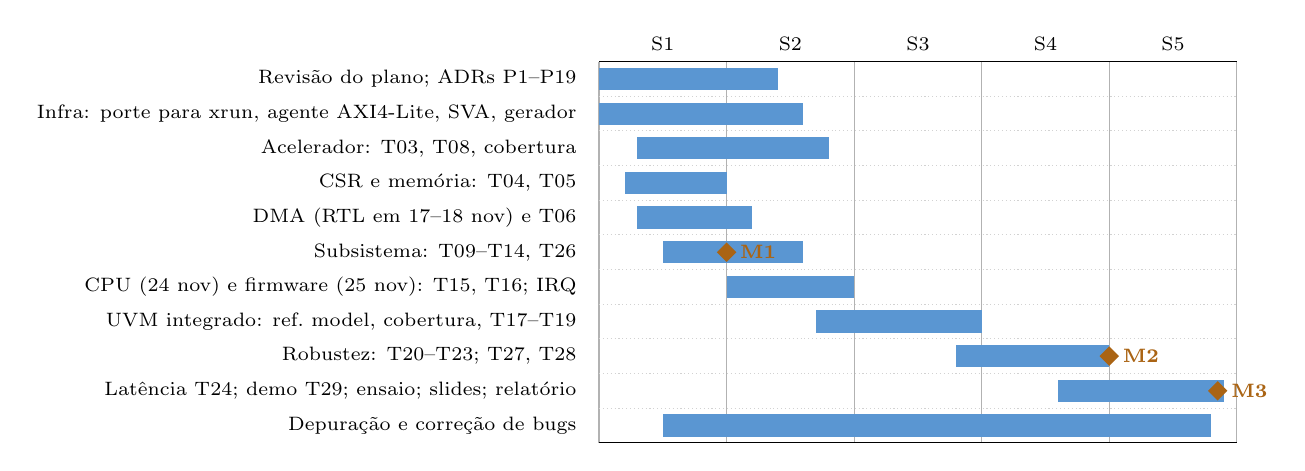
\begin{tikzpicture}[x=1.62cm,y=0.44cm,font=\scriptsize]
\foreach \i/\n in {0/S1,1/S2,2/S3,3/S4,4/S5} {
  \node[anchor=south] at (\i+0.5,0.05) {\n};
  \draw[gray!60] (\i,0) -- (\i,-11);
}
\draw[gray!60] (5,0) -- (5,-11);
\draw (0,0) -- (5,0);
\draw (0,-11) -- (5,-11);
\foreach \r in {1,...,10} { \draw[gray!35,densely dotted] (0,-\r) -- (5,-\r); }
\foreach \r/\name/\s/\e in {
  1/{Revisão do plano; ADRs P1--P19}/0/1.4,
  2/{Infra: porte para xrun, agente AXI4-Lite, SVA, gerador}/0/1.6,
  3/{Acelerador: T03, T08, cobertura}/0.3/1.8,
  4/{CSR e memória: T04, T05}/0.2/1.0,
  5/{DMA (RTL em 17--18 nov) e T06}/0.3/1.2,
  6/{Subsistema: T09--T14, T26}/0.5/1.6,
  7/{CPU (24 nov) e firmware (25 nov): T15, T16; IRQ}/1.0/2.0,
  8/{UVM integrado: ref.\ model, cobertura, T17--T19}/1.7/3.0,
  9/{Robustez: T20--T23; T27, T28}/2.8/4.0,
  10/{Latência T24; demo T29; ensaio; slides; relatório}/3.6/4.9,
  11/{Depuração e correção de bugs}/0.5/4.8} {
  \node[anchor=east] at (-0.1,-\r+0.5) {\name};
  \fill[bar] (\s,-\r+0.18) rectangle (\e,-\r+0.82);
}
\foreach \x/\r/\m in {1.0/6/M1, 4.0/9/M2, 4.85/10/M3} {
  \node[diamond,fill=ms,inner sep=1.8pt] at (\x,-\r+0.5) {};
  \node[anchor=west,ms] at (\x+0.03,-\r+0.5) {\textbf{\m}};
}
\end{tikzpicture}
\caption{Cronograma preliminar (S1 = semana de 16/11/2026). M1 = tag \code{e3} (22/11); M2 = tag
\code{e4} (13/12); M3 = apresentação e demonstração (18--19/12).}
\label{fig:gantt}
\end{figure}

\begin{table}[htbp]
\centering\small
\caption{Etapas, datas e entregáveis.}
\label{tab:etapas}
\begin{tabular}{@{}L{1.2cm}L{2.2cm}L{11.7cm}@{}}
\toprule
Semana & Período & Atividades e entregáveis\\
\midrule
S1 & 16/11 -- 22/11 & Revisão do plano com a equipe; ADRs dos pontos bloqueantes (P1, P8, P9, P10,
P12, P13); ICD v1.1 com mapa de memória e registradores do DMA; porte do testbench do acelerador
para \code{xrun} e \code{make sim-accel}; T03; RTL e testbench do CSR e da memória (T04, T05); RTL
do DMA (17--18/11) e T06; ambiente de subsistema com driver A, agente AXI4-Lite e SVA; T09--T11;
regressão por seeds $\times$ $N$. \textbf{M1 (tag \code{e3}):} DMA, memória e acelerador aprovados
juntos.\\
S2 & 23/11 -- 29/11 & T12--T14; cobertura \code{cg\_axil}, \code{cg\_accel\_*}, \code{cg\_dma\_op};
T08; core (24/11) e firmware genérico (25/11) no \code{soc\_top}; T15 e T16 com driver B por
\emph{factory override}; decisão sobre interrupção (29/11); plano v0.2.\\
S3 & 30/11 -- 06/12 & UVM integrado completo: reference model por TLM, monitor de barramento,
\code{cg\_sys}; T17--T19; regressão nas três configurações; análise dos buracos de cobertura.
Relatórios de síntese dos blocos (06/12, fora deste plano).\\
S4 & 07/12 -- 13/12 & Robustez: T20 (se IRQ), T21--T23; T27 e T28; exclusões de cobertura
justificadas; README de verificação com os comandos de compilação, simulação e regressão.
\textbf{M2 (tag \code{e4}):} regressão final com vereditos e cobertura no IMC.\\
S5 & 14/12 -- 19/12 & T24 (latência para o comparativo de desempenho); T29 ensaiado no servidor da
disciplina, com gravação de contingência; seção de verificação do relatório; slides; tag
\code{final}. \textbf{M3:} apresentação e demonstração ao vivo (18--19/12).\\
\bottomrule
\end{tabular}
\end{table}

\paragraph{Riscos ao cronograma.}
\begin{enumerate}[label=(\roman*),leftmargin=2.6em]
  \item \textbf{RTL ainda não escrito} (DMA, CSR, memória, core, \code{soc\_top}). Mitigação:
  modelos comportamentais e driver A permitem fechar o ambiente antes; cada teste entra quando o RTL
  chega.
  \item \textbf{ICD incompleto} (P9, P10) bloqueia firmware, decodificador e ambiente. Mitigação:
  ADRs na S1; header do firmware gerado de uma fonte única.
  \item \textbf{Decisão de tiling} (P1, P2, P12) muda a FSM do DMA e o scoreboard. Mitigação:
  decidir na S1; scoreboard parametrizado pelo \emph{wrap}.
  \item \textbf{Toolchain e licenças}: testbench em Vivado, Xcelium e IMC licenciados, ausência de
  toolchain RISC-V no servidor. Mitigação: \code{env\_smoke} já prova \code{xrun} + UVM;
  \code{.hex} versionado; porte do testbench na S1.
  \item \textbf{Tempo de simulação} com $N = 8$ e vários tiles no nível de sistema. Mitigação:
  limitar dimensões no aleatório de sistema; dimensões grandes só no subsistema; regressão noturna.
  \item \textbf{Core RV32I}: se próprio e atrasado, a demonstração do top-level fica sem firmware.
  Mitigação: ADR com core de terceiros como alternativa; o driver A mantém o restante verificado.
  \item \textbf{Demonstração ao vivo}: falha de servidor ou de licença. Mitigação: ensaio no mesmo
  servidor e com o mesmo usuário; gravação de tela como contingência.
\end{enumerate}

% ------------------------------------------------------------------ refs
\begin{thebibliography}{9}
\bibitem{piziali} A. Piziali. \emph{Functional Verification Coverage Measurement and Analysis}.
Springer, 2004.
\bibitem{vmm} J. Bergeron, E. Cerny, A. Hunter, A. Nightingale. \emph{Verification Methodology
Manual for SystemVerilog}. Springer, 2005.
\bibitem{uvm} Accellera. \emph{Universal Verification Methodology (UVM) 1.2 User's Guide}, 2015;
IEEE Std 1800.2-2020.
\bibitem{sv} IEEE Std 1800-2017. \emph{SystemVerilog --- Unified Hardware Design, Specification,
and Verification Language}.
\bibitem{axi} Arm. \emph{AMBA AXI and ACE Protocol Specification} (AXI4-Lite).
\bibitem{riscv} RISC-V International. \emph{The RISC-V Instruction Set Manual, Volume I:
Unprivileged ISA}.
\bibitem{kung} H. T. Kung. Why systolic architectures? \emph{IEEE Computer}, 15(1), 1982.
\bibitem{enunciado} CEPEDI / CI Digital. \emph{RISC-V com Coprocessador de Multiplicação Matricial
e Controlador DMA} (enunciado do projeto final) e \emph{SD242 --- Ambiente UVM para o top-level
RISC-V + DMA + Systolic Array} (trabalho final de verificação).
\bibitem{repo} Repositório \code{riscv-dma-matrix-coprocessor}: \code{README.md},
\code{CONTRIBUTING.md}, \code{02.Architecture/roadmap.md}, \code{02.Architecture/icd/csr\_readme.md},
\code{04.RTL/accel/readme.md}.
\end{thebibliography}

\end{document}
